\section{Dataset and Preprocessing}
\label{sec:method-dataset}

\subsection{Dataset}
\label{sec:method-dataset-generation}

We construct a binary classification dataset of benign Coyote partial bitstreams
and malicious RO-based partial bitstreams generated through the Coyote
partial-reconfiguration flow. The benign class contains eight Coyote applications
spanning HLS, cryptographic, communication, and compute examples. We build
these applications across multiple Coyote floorplans, yielding 221 benign partial
bitstreams.

Malicious samples use the RO-based designs of Mahmoud
et al.~\cite{mahmoud2023practical}, instantiated at different payload sizes and
floorplans. The main corpus contains 225 malicious partial bitstreams. We
additionally generate 78 higher-density samples, excluded from training and used
only for the RO-footprint evaluation. Figure~\ref{fig:ro-count-distribution}
shows the RO-count distribution of the main malicious dataset and its
higher-density extension.

\begin{figure}[tbp]
\centering
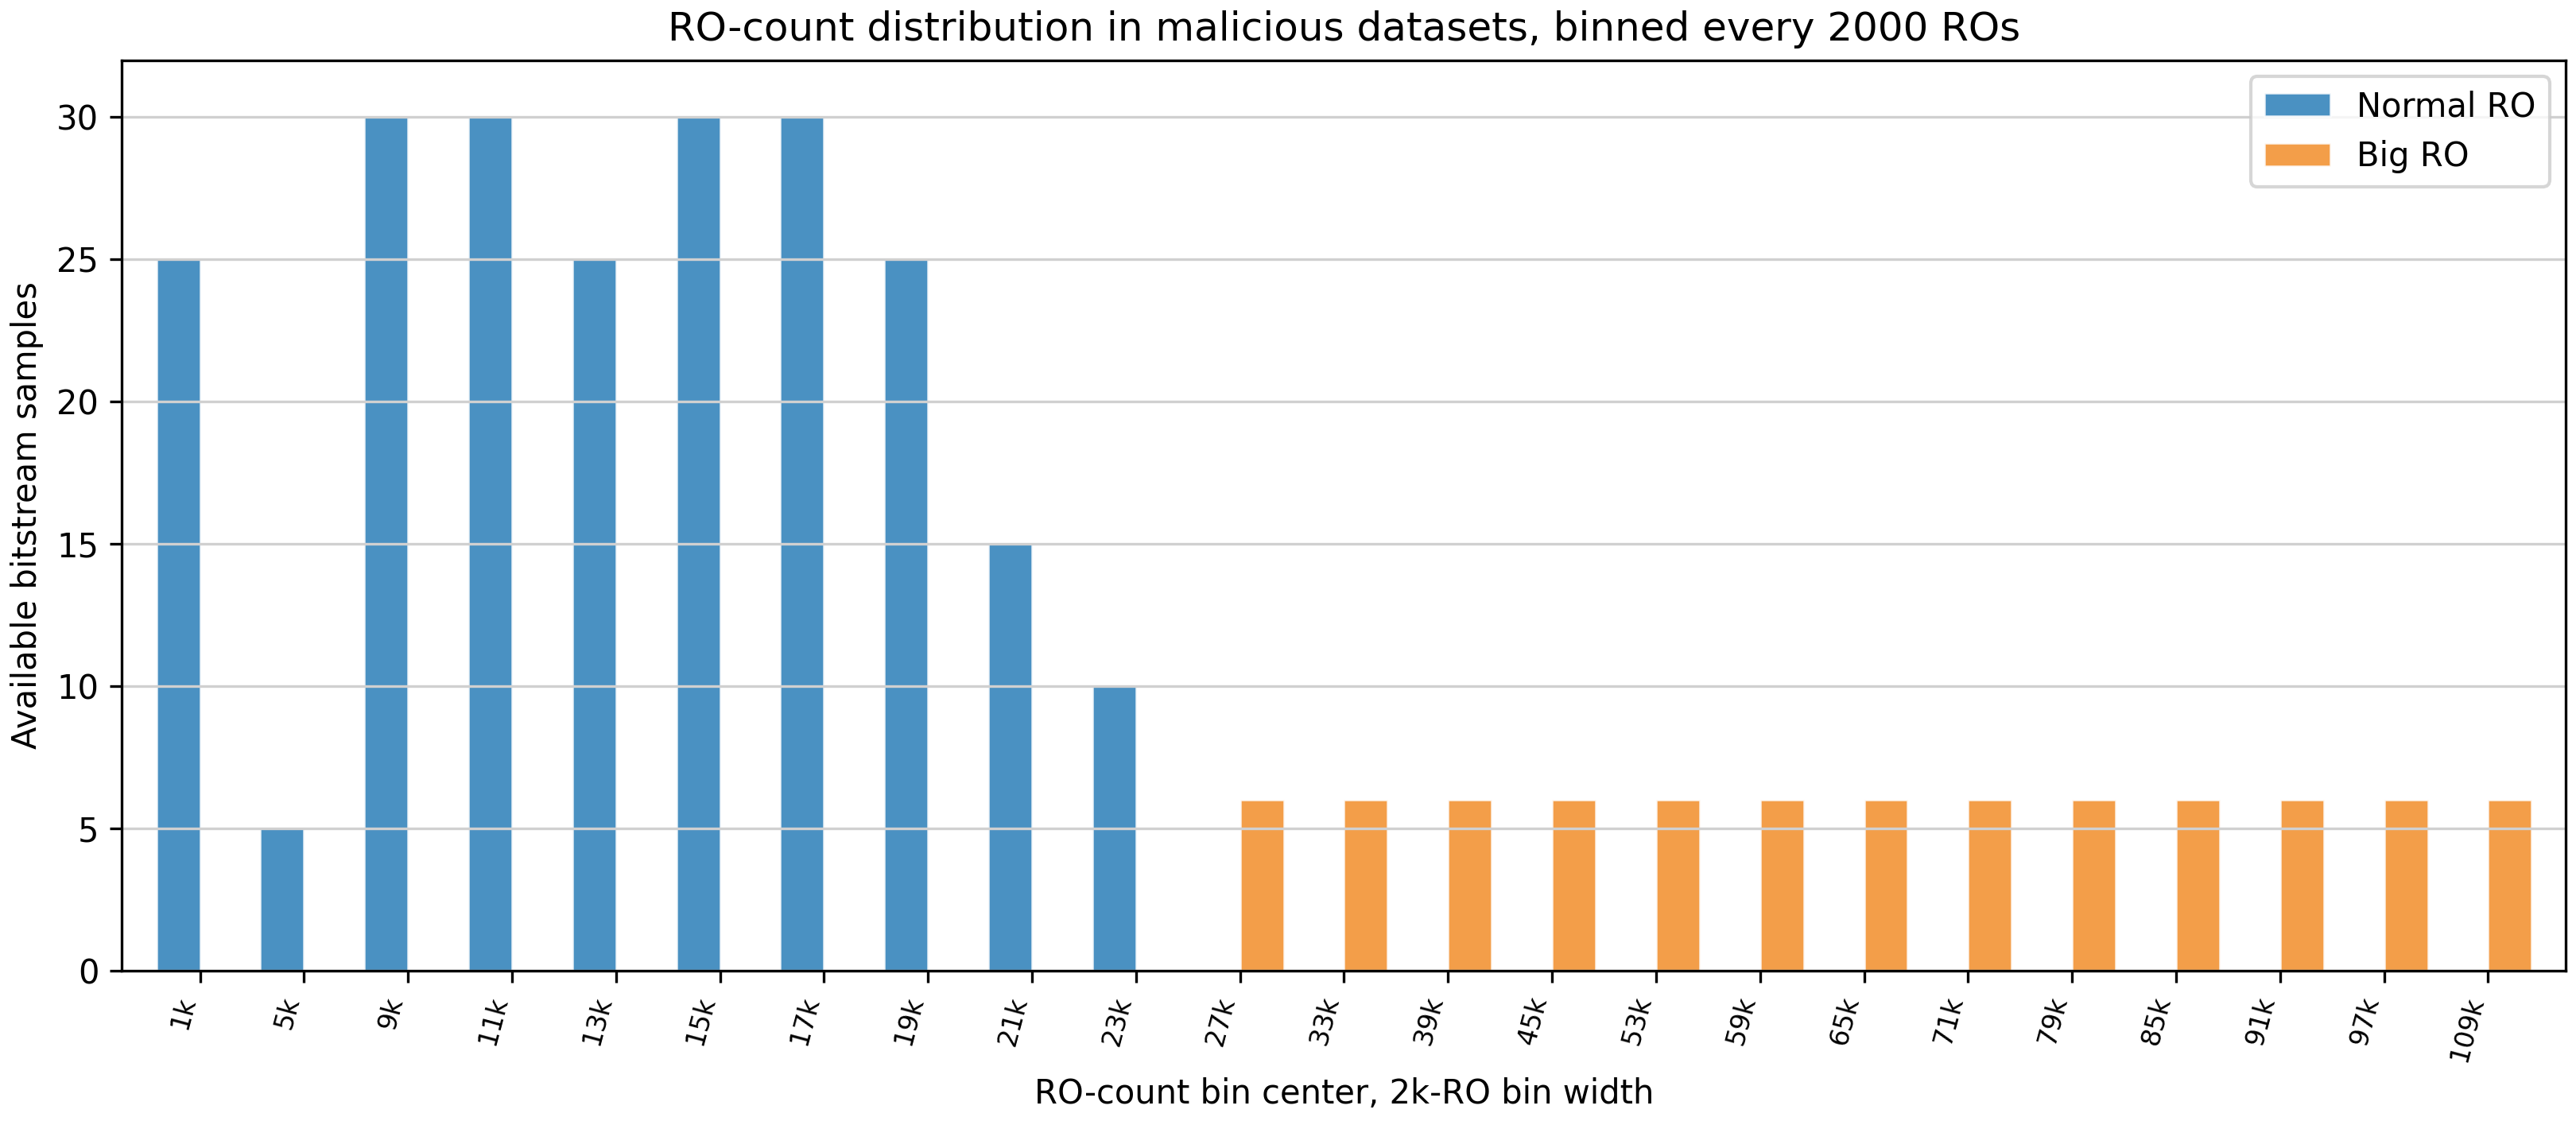
\includegraphics[width=0.95\linewidth]{figures/ro_count_distribution.png}
\caption{Distribution of RO counts in the normal-RO dataset and the big-RO
extension. Bars count available bitstream samples in 2k-RO bins.}
\label{fig:ro-count-distribution}
\end{figure}

\subsection{Preprocessing}
\label{sec:method-preprocessing}

We map each raw partial bitstream to a fixed-size
$H \times W \times 1$ tensor using Algorithm~\ref{alg:preprocessing}. The
transformation uniformly samples or pads the byte stream to $H \cdot W$ bytes,
then inverts, normalizes, and reshapes the selected values.

\begin{algorithm}[t]
\caption{Deterministic bitstream preprocessing.}
\label{alg:preprocessing}
\begin{algorithmic}[1]
\Require Bitstream bytes $b$, target dimensions $H$, $W$
\State $T \gets H \cdot W$
\If{$|b| > T$}
\State $i \gets \left\lfloor \operatorname{linspace}(0, |b|-1, T) \right\rfloor$
\State $b \gets b[i]$
\Else
\State $b \gets \operatorname{ZeroPad}(b, T)$
\EndIf
\State $x \gets \operatorname{Reshape}((255-b)/255, H, W, 1)$
\State \Return $x$
\end{algorithmic}
\end{algorithm}

Our final checker uses a $256 \times 256$ input, corresponding to 65,536 sampled
bytes per partial bitstream. We evaluate additional input resolutions during the
model design-space exploration in Section~\ref{sec:ml-inspection}.
